\documentclass[../report.tex]{subfiles}
\graphicspath{{\subfix{../image/}}}

\begin{document}

\subsection{Power Supply}
Providing power is essential for the forklift to work. The power supply (circuit)
needs to fulfill the following requirements:
\begin{itemize}
    \item Provide voltage and current to motors
    \item Provide voltage and current to IC (from loadcell-PCB to ESP32)
    \item Long-living
    \item Weight is not important as counterweight is needed
\end{itemize} 
\subsubsection{The Supply - the battery}
The maximum voltage required by the forklift is 12V. This is for the motors. As the forklift
is not stationary a 12V battery is required. The choice is a 12V lead-acid 
battery by RS. It can supply the motor currents, has a high capacity (7Ah) and can serve as a counterweight (2.2 kg).
Uni had it stock: \url{https://dk.rs-online.com/web/p/blybatterier/5375488}
\subsubsection{The Supply Circuit}
12V is not the only voltage level required. 5V is needed by the IR-sensors and the ESP32. And 3.3V is required
by the loadcell-amplification-circuit. 
\begin{figure}[h!]
    \centering
    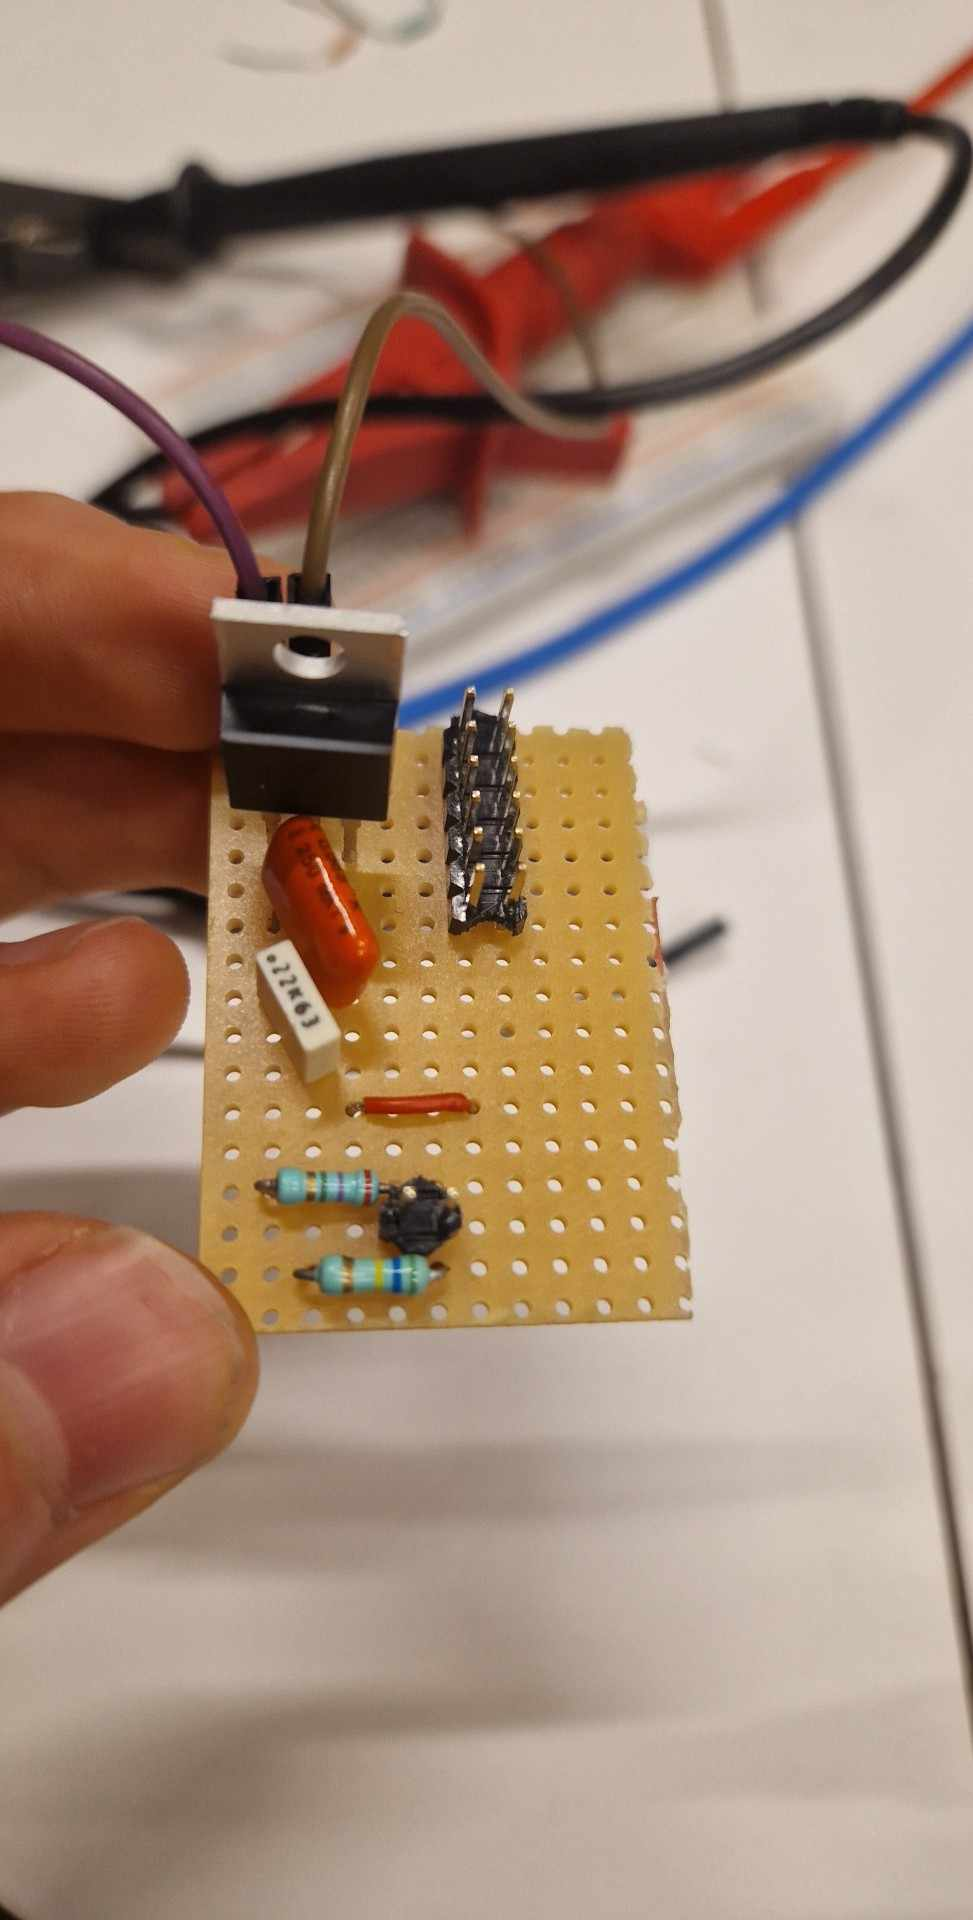
\includegraphics[width=0.2\textwidth]{powerregcircuit.jpg}
    \caption{Power Regulator Circuit + Voltage divider for battery voltage}
 \end{figure}
The ESP32 has an on-board 3.3V-regulator. Thus, by supplying 5V to the ESP, the 3.3V-level is given.
To achieve the 5V the TS-7805 voltage regulator is used. Alone it can supply a current of 1A at maximum, which
is enough to power the microcontroller and the IR-sensors and multiplexers. Moreover, two analog filters are required
for the circuit to work. There are two low pass filters: One in the output of 0.1µF and one of 0.33µF in the input.
These values are determined by the datasheet. As 0.33µF was not in stock at the labs - capacitors were 
soldered in parallel in order to achieve a capacitance of 0.3µF. The reliability of this setup
has been tested on a breadboard before.

A later adjustment of the board was adding a big ground rail to the right side.
\end{document}